\section{Classification Storage API}
    Wie werden die Daten in die DB geschrieben bzw. gelesen.

    \subsection{Funktionen und Schnitstellen}

    \subsection{Was ist eine Seite}
        \begin{figure}
            \centering
            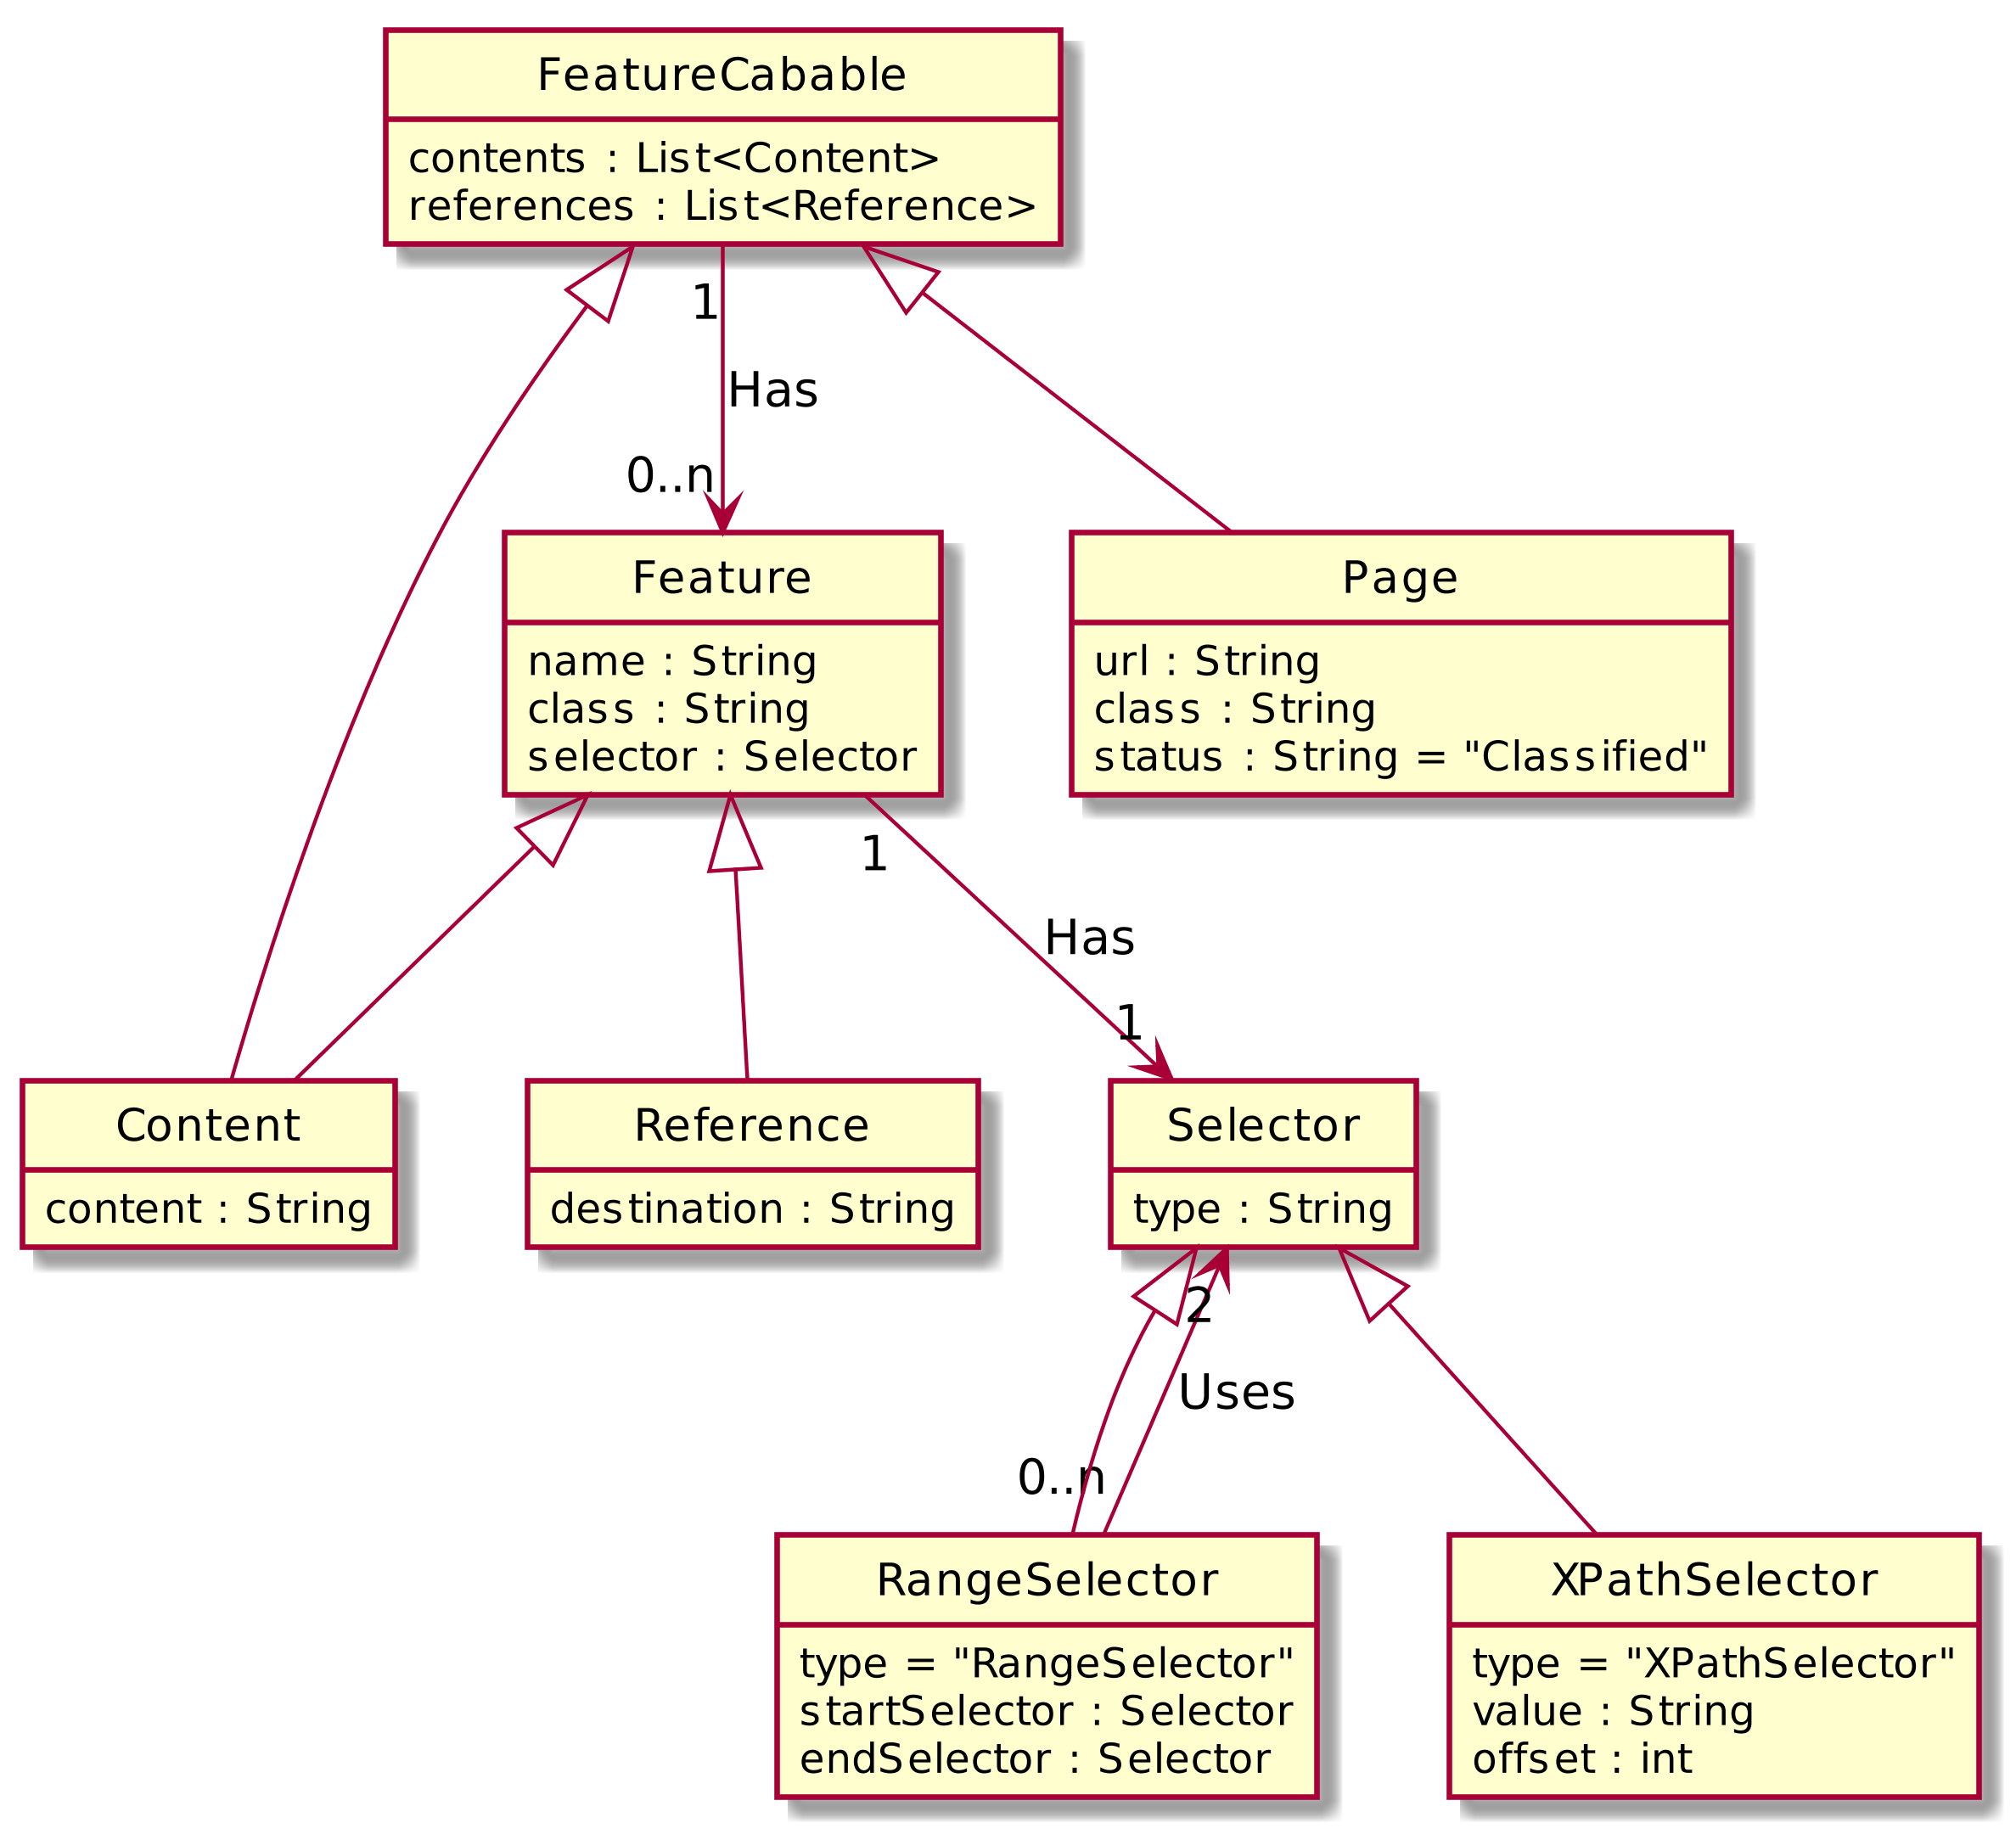
\includegraphics[width=\textwidth]{../resources/storage-api-data-model/page.png}
            \caption{Seite in der Storage API}
            \label{image:storageApiPageModel}
        \end{figure}

    \subsection{Algorithmus zum (initialen) ANLEGEN}
        \lstinputlisting[label=listing:storeClassification,caption=Algorithmus zum Speichern]{../resources/store-classification.code}